\documentclass{article}

%other packages
\usepackage[a4paper]{geometry}
\usepackage{longtable}
\usepackage{wrapfig}
\setlength\parindent{0pt}
\usepackage{enumitem}
\usepackage[table]{xcolor}
\usepackage{polynom}
\def\scaleint#1{\vcenter{\hbox{\scaleto[3ex]{\displaystyle\int}{#1}}}}
\usepackage{array}
\newcolumntype{C}{>{{}}c<{{}}} % for '+' and '-' symbols
\newcolumntype{R}{>{\displaystyle}r} % automatic display-style math mode 
\usepackage{tabularray}
\usepackage{dcolumn,tabularx,booktabs}

%maths
\usepackage{mathtools}
\usepackage{amsmath}
\usepackage{amssymb}
\usepackage{amsfonts}
\usepackage{autobreak}

%tikzpicture
\usepackage{tikz}
\usepackage{scalerel}
\usepackage{pict2e}
\usepackage{tkz-euclide}
\usepackage{tikz-3dplot}
\usetikzlibrary{calc}
\usetikzlibrary{patterns,arrows.meta}
\usetikzlibrary{shadows}
\usetikzlibrary{external}
\usetikzlibrary{decorations.pathreplacing,angles,quotes}

%pgfplots
\usepackage{pgfplots}
\pgfplotsset{compat=1.18}
\usepgfplotslibrary{statistics}
\usepgfplotslibrary{fillbetween}

\pgfplotsset{
    standard/.style={
    axis line style = thick,
    trig format=rad,
    enlargelimits,
    axis x line=middle,
    axis y line=middle,
    enlarge x limits=0.15,
    enlarge y limits=0.15,
    every axis x label/.style={at={(current axis.right of origin)},anchor=north west},
    every axis y label/.style={at={(current axis.above origin)},anchor=south east}
    }
}

\begin{document}

Math 115 - Week 1, Class 1 - 3 Jan 2024
\hrule

\begin{center}
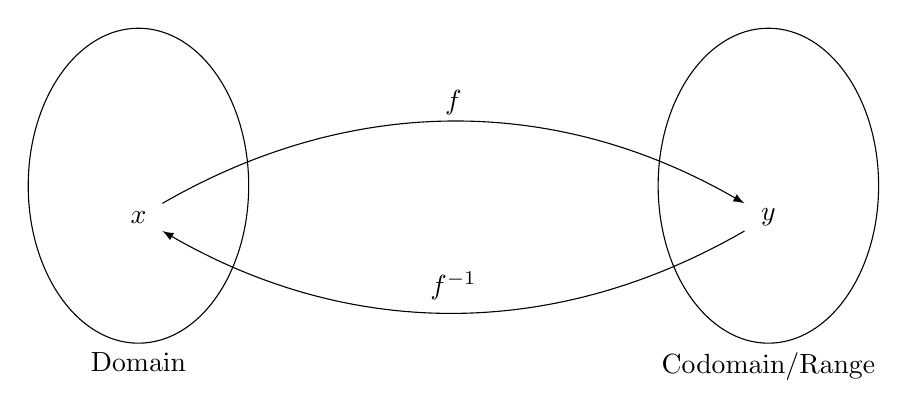
\begin{tikzpicture}[scale=2]
\draw (-2,0) circle [x radius=0.7, y radius=1];
\node[below] at (-2,-1) {Domain};
\node at (-2,-0.2) {$x$};
\draw(2,0) circle [x radius=0.7, y radius=1];
\node[below] at (2,-1) {Codomain/Range};
\node at (2,-0.2) {$y$};
%arrows
\draw[-latex,shorten <=10,shorten >=10] (-2,-0.2) to[bend left] node[midway,above]{$f$} (2,-0.2);
\draw[latex-,shorten <=10,shorten >=10] (-2,-0.2) to[bend right] node[midway,above]{$f^{-1}$} (2,-0.2);
\end{tikzpicture}
\end{center}

For every $x$ in the domain of $f$, there exists a $y=f(x)$ such that $x\in\mathbb{R}$ and $y\in\mathbb{R}$.

\begin{center}
\begin{tabular}{|ll|}
\hline&\\
\multicolumn{2}{|l|}{{\bf{}Terminology}}\\[0.5em]
$x$ - independent variable & "$y$ is the image of $x$"\\[0.5em]
$y$ - the value of the function & "$x$ is a pre-image of $y$"\\[1em]
\hline
\end{tabular}
\end{center}

Take $y=x^2$, for example. For every $y\geq0$, there are two pre-images: $x_1=\sqrt{y}$ and $x_2=-\sqrt{y}$.

\vspace{10pt}

\begin{tabularx}{\textwidth}{|X|}
\cline{1-1}\\
A function $f$ is called a {\bf{}one-to-one function} if it never takes on the same value twice; that is,\\[0.5em]
\multicolumn{1}{|c|}{$f(x_1)\neq f(x_2)\qquad\textnormal{whenever }x_1\neq x_2$}\\[1em]
\cline{1-1}
\end{tabularx}

\vspace{10pt}

Equivalently, a function $f$ is $1\to1$ if every image of $f$ has exactly one pre-image.

\vspace{10pt}

Also equivalently, $f$ is $1\to1$ if it is monotonic. That is, $x_1<x_2$ implies either $y_1<y_2$ or $y_1>y_2$ for all $x$ in the domain of $f$.

\vspace{10pt}

Now to \underline{the point}; if $f$ is a $1\to1$ function, then there exists an {\bf{}inverse function} denoted by $f^{-1}$. If a function maps $x$ into $y$, then its inverse function maps $y$ back into $x$. That is,

\begin{center}
\begin{tabular}{|c|}
\hline\\
$f^{-1}(f(x))=x$\\[1em]
\hline
\end{tabular}
$\longrightarrow\begin{array}{l}\textnormal{Must be satisfied for}\\ \textnormal{whole domain of inverse.}\end{array}$
\end{center}

The textbook gives this definition:

\vspace{10pt}

\begin{tabularx}{\textwidth}{|X|}
\cline{1-1}\\
Let $f$ be a one-to-one function with domain $A$ and range $B$. Then its {\bf{}inverse function} $f^{-1}$ has domain $B$ and range $A$ and is defined by\\[2em]
\multicolumn{1}{|c|}{$f^{-1}(y)=x\quad\Longleftrightarrow\quad f(x)=y$}\\[0.5em]
for any $y$ in $B$.\\[1em]
\cline{1-1}
\end{tabularx}

\vspace{10pt}

{\bf{}EXAMPLE} Given $f(x)=x^2-3x+1$, define $f^{-1}$. Restrict the domain if necessary.

\vspace{10pt}

First we solve for $x$ in terms of $y$. \[\textnormal{Let }y=f(x)\quad x=f^{-1}(y)\]

\begin{align*}
y&=x^2-3x+1\\
0&=x^2-3x+1-y\\
\textnormal{Generally, }x&=\frac{-b\pm\sqrt{b^2-4ac}}{2a}\\
\textnormal{But here, }x&=\frac{-b+\sqrt{b^2-4ac}}{2a}=\frac{3+\sqrt{4y+5}}{2}
\end{align*}

We write $+$ instead of $\pm$, restricting the range of $f^{-1}$ so that it abides by the definition of a function (ie. an input cannot have more than one output). Note that the choice of $+$ over $-$ was an arbitrary decision.

\vspace{10pt}

Finally, we verify that $f^{-1}(f(x))=x$.

\begin{align*}
f^{-1}(f(x))&=\frac{3}{2}+\sqrt{y+\frac{5}{4}}\\
&=\frac{3}{2}+\sqrt{\frac{5}{4}+x^2-3x+1}\\
&=\frac{3}{2}+\sqrt{\left(x-\frac{3}{2}\right)^2}\\
&=\frac{3}{2}+x-\frac{3}{2}=x
\end{align*}

{\bf{}EXAMPLE} Sketch $\sqrt[3]{1-x^3}\quad-\infty<x<\infty$

\vspace{10pt}

Our Math Professor recommmends analyzing the asymptotic behaviour first when sketching curves. A rigorous step-by-step prodecure for curve sketching (which includes asymptotic analysis, just not first) can be found in Stewart.

\vspace{10pt}

Asymptotic Analysis Strategy 1:

$x\to\infty\qquad x^3>>1$

Since $x^3>>1$, we can neglect the 1 and say $y\sim\sqrt[3]{-x^3}=-x\textnormal{ where }y>-x$

\vspace{10pt}

Asymptotic Analysis Strategy 2:

$y=\sqrt[3]{1-x^3}=\sqrt[3]{(-x)^3(1-1/x^3)}=-x\sqrt[3]{1-\frac{1}{x^3}}$

and since $\sqrt[3]{1-\frac{1}{x^3}}$ tends to 1, $y\sim-x$

\vspace{10pt}

In this example, after the asymptotic analysis, Our Math Professor checked the $x$ and $y$-intercepts.

When $x=0$, $y=1$. And when $y=0$, $x=1$.

\vspace{10pt}

In this example, these two forms of curve analysis have given us enough information to draw the curve. I feel that it's important to note that different functions have different idiosyncracies, and may require different forms of analysis to sketch. But anyways, here's the finished product!

\begin{center}
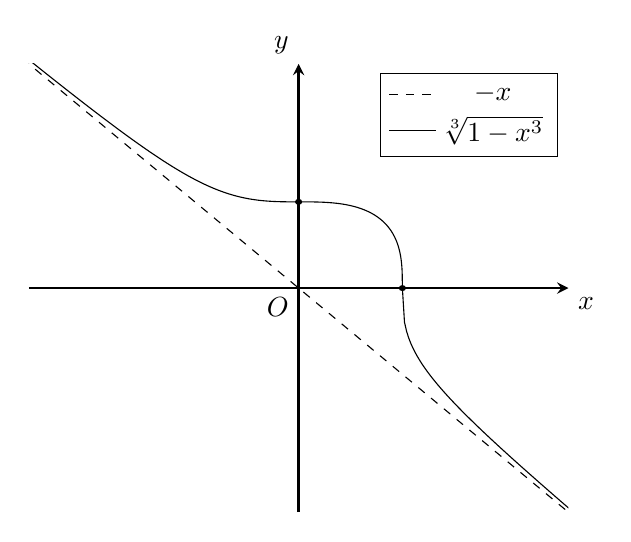
\begin{tikzpicture}
\begin{axis}[
standard,
xmin=-2, xmax=2,
ymin=-2, ymax=2,
xtick={\empty}, ytick={\empty},
xlabel={$x$}, ylabel={$y$}]
\addplot[dashed]{-x};\addlegendentry{\(-x\)}
\addplot[samples=100,domain=-3:0]{-x*(1-1/x^3)^(1/3)};
\addplot[samples=500,domain=0:1]{(1-x^3)^(1/3)};\addlegendentry{\(\sqrt[3]{1-x^3}\)}
\addplot[samples=100,domain=1:3]{-x*(1-1/x^3)^(1/3)};
\node[below left] at (0,0) {$O$};
\fill (0,1) circle [radius=0.035];
\fill (1,0) circle [radius=0.035];
\end{axis}
\end{tikzpicture}
\end{center}


\end{document}